\section{Étude de la station totale LeICA TCra 1103 \label{CCS_MP_2017:p4}}
\subsection{Mesure par une station totale et exigences client}

\ifprof
\else
Dans une station totale, les deux axes d'azimut et d'élévation, motorisés et asservis en position angulaire, poursuivent en continu le prisme rétro-réfléchissant déplacé par l'opérateur : dès que ce dernier s'immobilise au point qu'il a choisi pour effectuer une mesure, le système de visée recale le faisceau au centre du prisme (cette opération dure moins d'une seconde) et informe l'opérateur qui peut alors déclencher la mesure à distance\\
La station totale LeIcA TCRA 1103 est principalement composée de trois ensembles rigides en mouvements relatifs : le bâti $\underline{\mathbf{0}}$, la fourche d'azimut $\underline{\mathbf{1}}$ et le bloc optique $\underline{\mathbf{2}}$ (figure \ref{CCS_MP_2017:fig_02} et figure \ref{CCS_MP_2017:fig_06})\\

\begin{figure}[!h]
\centering
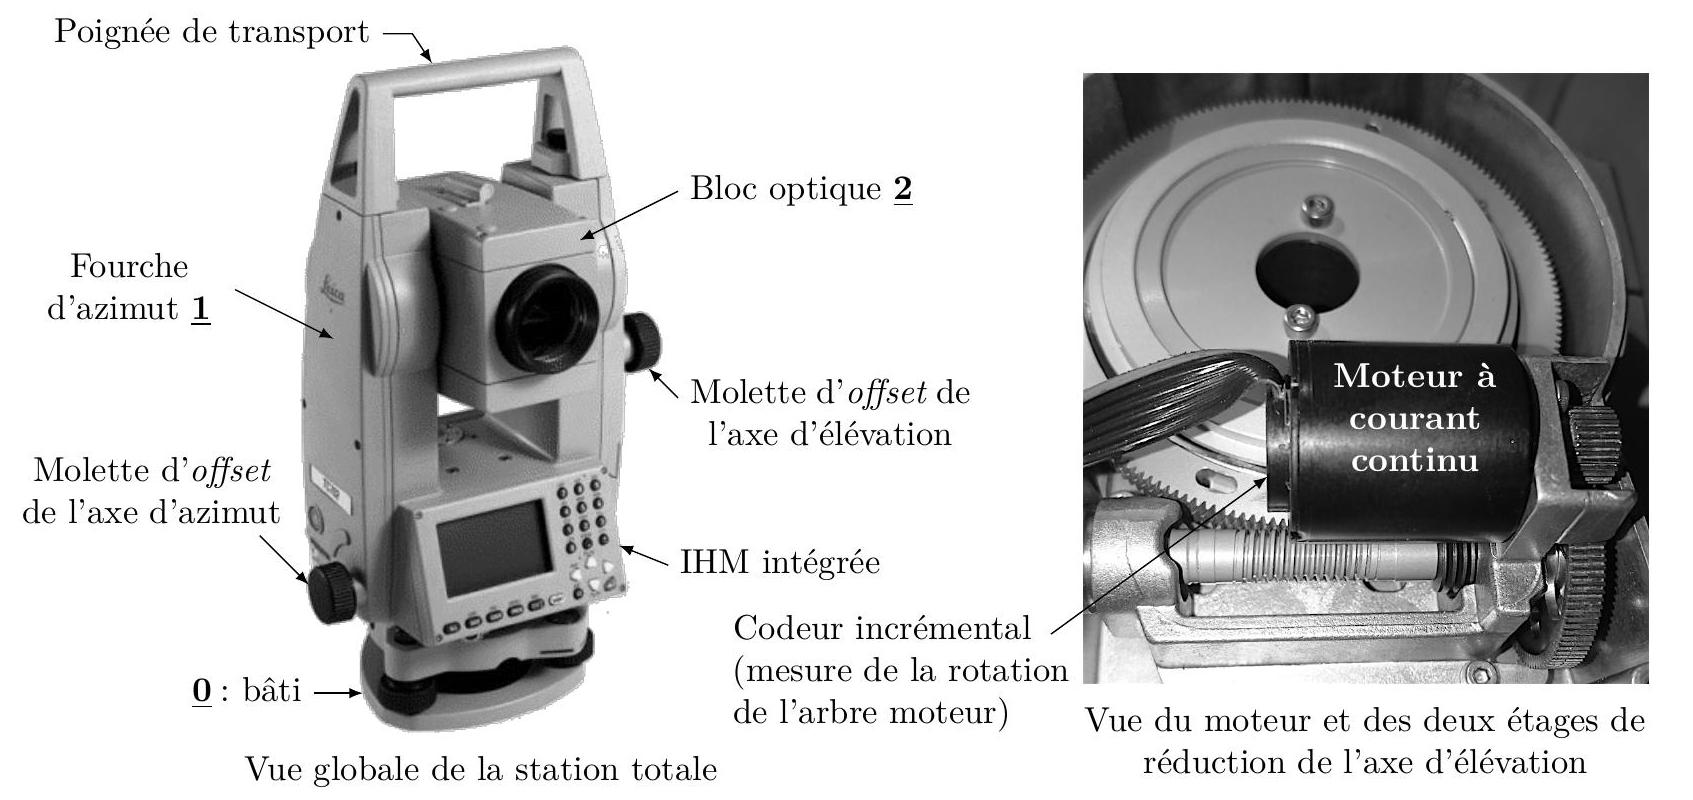
\includegraphics[width=\textwidth]{2024_12_07_51b7f57c7f055c2d8d29g-04(2)}

%Figure 6 
\caption{Photographies de la station totale LeICA TCRA 1103 \label{CCS_MP_2017:fig_06}}
\end{figure}

Les deux axes motorisés sont asservis en position angulaire: la description en chaines fonctionnelles de chacun des deux axes d'azimut (angle $\varphi$ ) et d'élévation (angle $\theta$ ) est fournie figure \ref{CCS_MP_2017:fig_07} L'interface homme - machine (IHM) intégrée à la station totale est constituée d'un pupitre et d'un écran tactile L'IHM déportée dispose des mêmes fonctionnalités que l'IHM intégrée et permet la communication et le pilotage à distance\\

\begin{figure}[!h]
\centering
%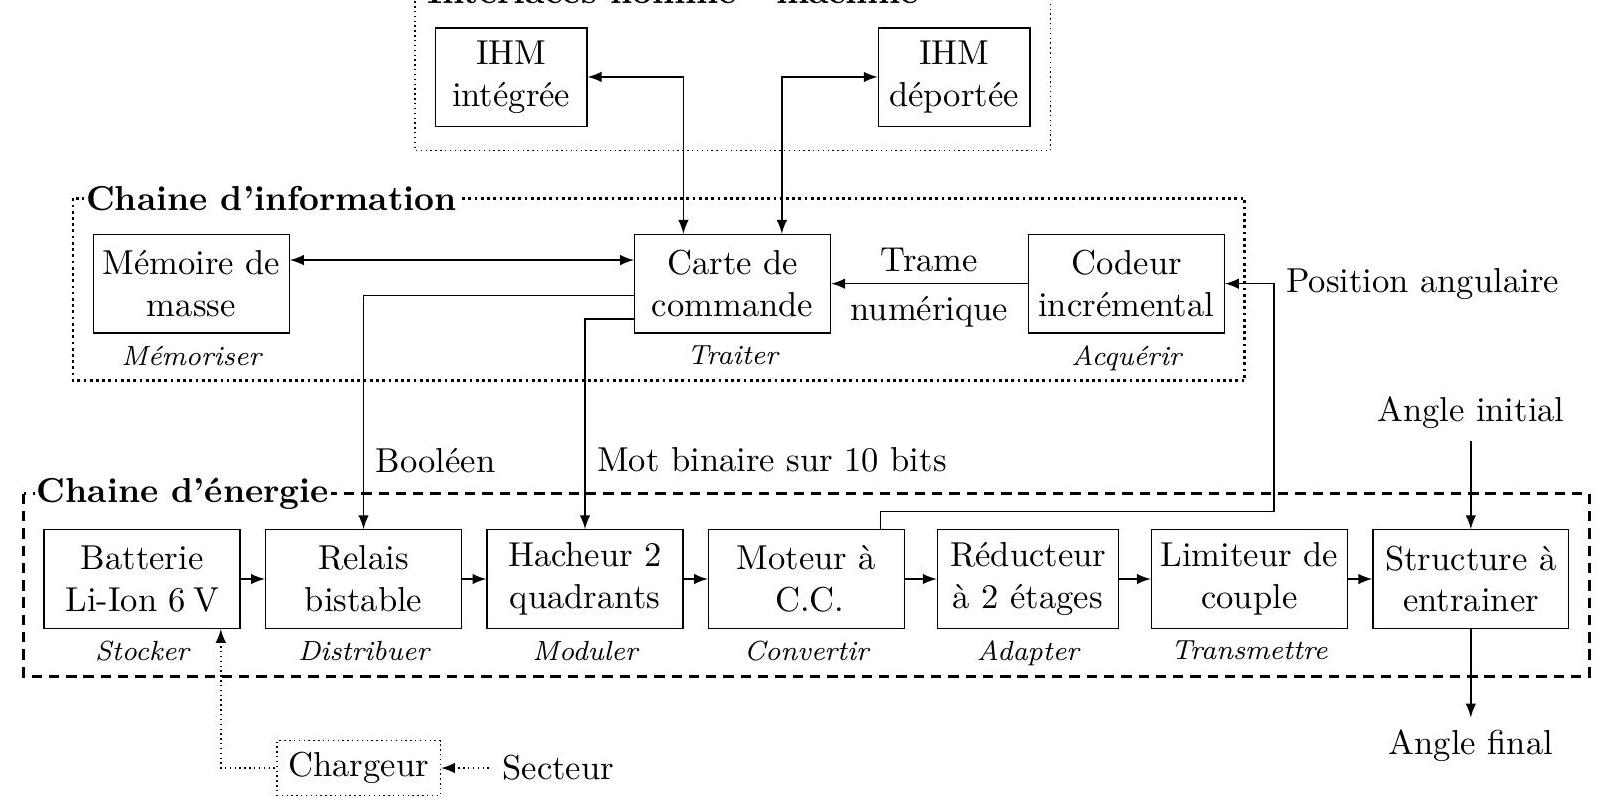
\includegraphics[width=\textwidth]{2024_12_07_51b7f57c7f055c2d8d29g-05}
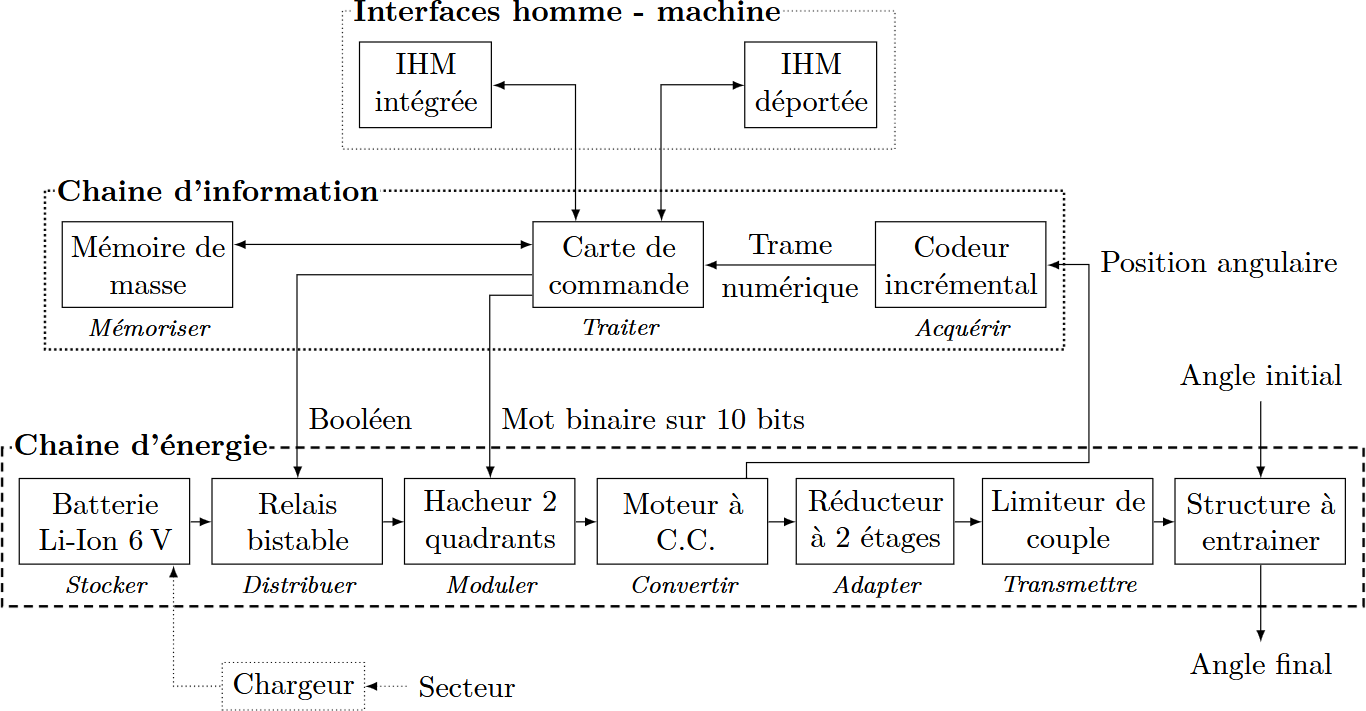
\includegraphics[width=\textwidth]{ccs_mp_2017_fig_07}

%Figure 7 
\caption{Description en chaines fonctionnelles de chacun des deux axes
\label{CCS_MP_2017:fig_07}}
\end{figure}

La mise en position de l'appareil (pointage du prisme optique rétro-réfléchissant) se fait de manière motorisée grâce au pupitre de commande Afin d'orienter plus rapidement l'axe de visée vers la cible, il est également possible de faire pivoter chacun des axes par action manuelle, comme dans le cas d'un théodolite : cette double fonctionnalité est permise par le limiteur de couple qui transmet la puissance du moteur à la structure à entrainer et glisse sous un effort manuel modéré de l'opérateur\\
Les exigences du point de vue des géomètres pour réaliser une mesure selon les normes ISO sont exprimées par l'exigence $\mathrm{Id}=  1  $ et ses deux sous-exigences $\mathrm{Id}=  11  $ et $\mathrm{Id}=  12  $ du diagramme partiel des exigences de la figure \ref{CCS_MP_2017:fig_08} Les sous-exigences $\mathrm{Id}=  11 1  , \mathrm{Id}=  12 1  $ et $\mathrm{Id}=  12 2  $ correspondent aux performances de la station totale Leica tcra 1103 telles que précisées dans son document technique



\begin{figure}[!h]
\centering
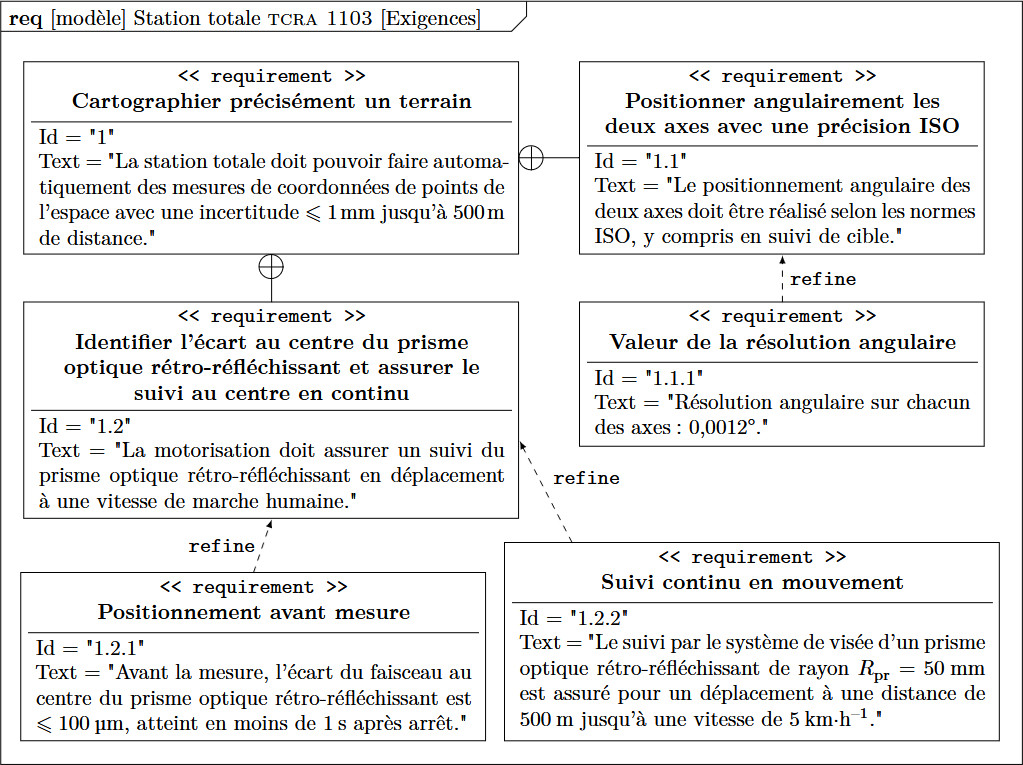
\includegraphics[width=.95\textwidth]{ccs_mp_2017_fig_08}

%Figure 0
\caption{Diagramme partiel des exigences de la station totale Leica\label{CCS_MP_2017:fig_08}}
\end{figure}
\fi

\subsection{Etude partielle de l’exigence Id =  11  « Positionner angulairement les deux axes avec
une précision ISO »}
\ifprof
\else

\begin{obj}
Vérifier la capacité de positionnement angulaire des axes
\end{obj}

Le processus de mesures en continu à l'aide de la station totale LEICA TCRa 1103 se compose de trois phases :

\begin{itemize}
  \item le suivi de la cible (le prisme optique rétro-réfléchissant) déplacée par l'opérateur ;
  \item le recalage de la ligne de visée sur le centre de la cible lors de l'arrêt du déplacement ;
  \item et la réalisation de la mesure
\end{itemize}

Afin de pouvoir effectuer une mesure au moment et au point souhaités, le rayon réfléchi par le prisme optique rétro-réfléchissant doit être continûment reçu par la station totale lors du déplacement de l'opérateur, quelles que soient les variations de vitesse de déplacement dues aux irrégularités du sol entre deux points de mesure Pour cela, le faisceau émis doit intercepter en permanence le prisme optique rétro-réfléchissant et le décalage angulaire lors du déplacement doit donc rester suffisamment faible pour garantir la réflexion

L'étude est limitée au cas où l'axe médian du prisme optique rétro-réfléchissant est situé dans le plan horizontal contenant la ligne de visée de l'optique : dans cette configuration, seul l'axe d'azimut est alimenté (l'étude serait identique pour l'analyse de l'axe d'élévation seul ou pour l'analyse de la commande couplée des deux axes)

Afin de garantir le respect des exigences de la station totale, le faisceau laser doit continûment pointer vers le prisme optique rétro-réfléchissant, ce qui implique:

\begin{itemize}
  \item une vitesse angulaire suffisamment importante pour pouvoir suivre tout déplacement de l'opérateur ;
  \item et un positionnement angulaire suffisamment précis pour assurer une mesure de qualité
\end{itemize}

La station totale TCRA 1103 est utilisée en topographie pour des distances comprises entre $D_{\text {mini }}=1,5 \mathrm{~m}$ et $D_{\text {maxi }}=500 \mathrm{~m}$ Le système de visée doit suivre l'opérateur qui déplace le prisme optique rétro-réfléchissant, de rayon $R_{\mathrm{Pr}}=50 \mathrm{~mm}$ (figure A du document réponse), à une vitesse maximale $V_{\mathrm{maxi}}=5 \mathrm{~km} \cdot \mathrm{~h}^{-1}$\\
La mesure est réalisée lorsque le faisceau laser pointe au centre du prisme optique rétro-réfléchissant, l'écart initial dû au suivi étant compensé avant toute mesure\\
\fi


%Q 6 
\question{\label{CCS_MP_2017:q_06}
Déterminer, en fonction des données, les expressions littérales puis calculer les valeurs numériques de la vitesse
 angulaire $\dot{\varphi}_{\mathrm{ref}}\left(\mathrm{entr} \cdot \mathrm{min}^{-1}\right)$ et de la résolution 
 angulaire $\Delta \varphi_{\mathrm{ref}}$ (en degrés) en azimut permettant d'assurer le suivi de l'opérateur 
 lorsqu'il déplace le prisme optique rétro réfléchissant entre deux mesures.}


\ifprof
\begin{corrige}
La vitesse de déplacement du point de mesure (F) (défini à la question 3 du corrigé), situé à une distance $D$ de l’isocentre, s’exprime par la relation : $V=D\varphip$Cette vitesse doit correspondre à la vitesse de déplacement de l’opérateur 

On se place dans le cas le plus défavorable pour la vitesse angulaire : $D=\indice{D}{mini} = \SI{1,5}{m}$ 
$\indice{\varphi}{Maxi} = \dfrac{\indice{V}{Maxi}}{{D}{mini}}$ en \si{rads^{-1}};  où 
$\indice{\varphip}{ref} = \dfrac{\indice{V}{Maxi}}{\indice{D}{Mini}} \dfrac{60}{2\pi}$ en \si{trmin^{-1}}

AN : $\indice{\varphip}{ref} = \dfrac{5\cdot 10^3 }{60\cdot 60\cdot 1,5} \dfrac{60}{2\pi} =\SI{8,84}{tr/min}$

Pour être certain que le système de visée suive le prisme optique, il faut que le rayon du prisme soit, au minimum, entièrement compris dans la résolution angulaire $\Delta \indice{\varphi}{ref}$ (voir figure)
On se place dans le cas le plus défavorable : $D=\indice{D}{Maxi} =\SI{500}{m}$ :  
$\tan(\Delta \indice{\varphi}{ref})=\dfrac{R_{Pr}}{D}$ et $\Delta \indice{\varphi}{ref}=\arctan\left(\dfrac{R_{Pr}}{\indice{D}{Maxi}}\right)$
AN  $\Delta \indice{\varphi}{ref}=\arctan(0,05/500)=5,7310^{(-3)}\degres =110^{(-4)} \si{rad}$

\end{corrige}
\else
\fi


\subsection{Étude partielle de l'exigence 12 : << Identifier l'écart au centre du prisme optique rétro-réfléchissant et assurer le suivi au centre en continu >>}

\ifprof
\else
\begin{obj}
Développer un modèle de simulation afin de mettre en œuvre une synthèse des lois de commande permettant de réaliser des mesures en continu avec une précision conforme aux attentes des géomètres
\end{obj}

\subsubsection{Données pour l'étude dynamique}
Le modèle choisi pour l'étude dynamique est fourni figure \ref{CCS_MP_2017:fig_09} \\


\begin{figure}[!h]
\centering
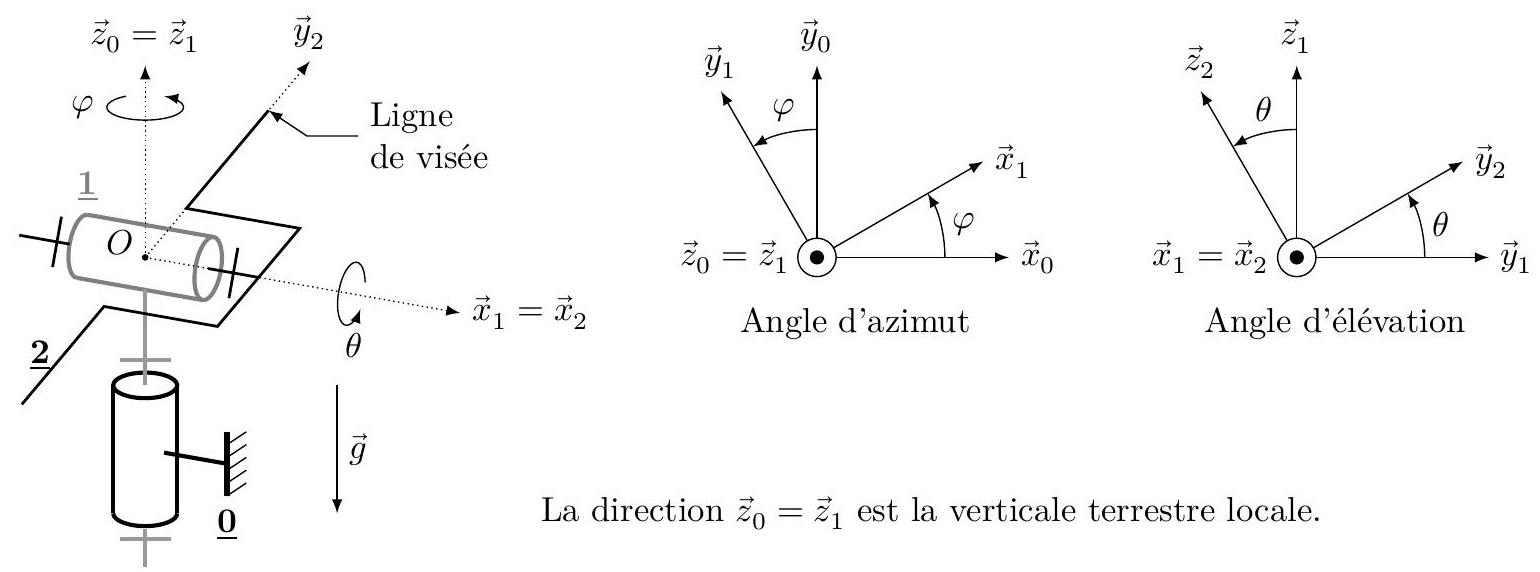
\includegraphics[width=\textwidth]{2024_12_07_51b7f57c7f055c2d8d29g-06}

%Figure 9 
\caption{Modèle géométrique de la partie mécanique de la station totale \label{CCS_MP_2017:fig_09}}
\end{figure}

Dans ce modèle, la fourche d'azimut $\underline{\mathbf{1}}$ ainsi que le bloc optique $\underline{\mathbf{2}}$ sont en mouvements relatifs par rapport au bâti $\underline{\mathbf{0}}$, supposé fixe par rapport à la terre Le repère $R\left(O ; \vec{x}_{0}, \vec{y}_{0}, \vec{z}_{0}\right)$ lié au bâti $\underline{\mathbf{0}}$ est galiléen L'accélération de la pesanteur $\vec{g}$ est selon la verticale terrestre locale (figure \ref{CCS_MP_2017:fig_09})

\begin{figure}[!h]
\centering
\begin{tabular}{lcc}
\hline
\textbf{Grandeurs} & \textbf{Fourche d'azimut 1} & \textbf{Bloc optique 2} \\
\hline
Repère associé $R_{i}\left(O ; \vec{x}_{i}, \vec{y}_{i}, \vec{z}_{i}\right)$ & $R_{1}\left(O ; \vec{x}_{1}, \vec{y}_{1}, \vec{z}_{1}\right)$ & $R_{2}\left(O ; \vec{x}_{2}, \vec{y}_{2}, \vec{z}_{2}\right)$ \\
Masse $M_{i}$ & $M_{1}$ & $M_{2}$ \\
Centre d'inertie $G_{i}$ & $G_{1} \equiv O$ & $G_{2} \equiv O$ \\
Matrice d'inertie $\mathbf{I}(O, i)$ exprimée & $\left[\begin{array}{ccc}J_{x 1} & 0 & 0 \\ 0 & J_{y 1} & 0 \\ 0 & 0 & J_{z 1}\end{array}\right]_{b_{1}}$ & $\left[\begin{array}{ccc}J_{x 2} & 0 & 0 \\ 0 & J_{y 2} & 0 \\ 0 & 0 & J_{z 2}\end{array}\right]_{b_{2}}$ \\
\hline
\end{tabular}
%Figure 10
\caption{Données géométriques et cinétiques associés aux deux pièces mobiles \label{CCS_MP_2017:fig_10}}
\end{figure}


Les deux axes asservis en azimut (angle $\varphi$ ) et en élévation (angle $\theta$ ) comportent chacun un réducteur de vitesse à deux étages et à rattrapage de jeu : un engrenage à dentures droites de rapport $\rho_{1 \mathrm{a}}$ (respectivement $\rho_{2 \mathrm{a}}$ ) suivi d'un engrenage à roue et vis sans fin de rapport $\rho_{1 \mathrm{~b}}$ (respectivement $\rho_{2 \mathrm{~b}}$ )\\
Les pertes en effort au niveau des axes de liaisons pivot sont modélisées par des facteurs de perte $k_{1}$ et $k_{2}$ (grandeurs sans unité, estimées par mesure), supposés constants dans toutes les configurations

\begin{figure}[!h]
\centering
\begin{tabular}{p{8cm}ll}
\hline
\textbf{Grandeurs} & \textbf{Liaison} $\boldsymbol{L}_{\mathbf{1 / 0}}$ & \textbf{Liaison} $\boldsymbol{L}_{\mathbf{2} / \mathbf{1}}$ \\
\hline
Modèle de liaison choisi & Pivot d'axe $\left(O, \vec{z}_{0}\right)$ & Pivot d'axe $\left(O, \vec{x}_{1}\right)$ \\

Paramètre angulaire & Angle d'azimut $\varphi$ & Angle d'élévation $\theta$ \\

Rapports des réducteurs de la liaison motorisée : & & \\

\begin{itemize}
\item étage a : réducteur à denture droite;
\end{itemize}
& $\dfrac{\omega_{1 / 0}}{\omega_{\mathrm{m} 1}}=\rho_{1 \mathrm{a}} \rho_{1 \mathrm{~b}}=\rho_{1}$ 
& $\dfrac{\omega_{2 / 1}}{\omega_{\mathrm{m} 2}}=\rho_{2 \mathrm{a}} \rho_{2 \mathrm{~b}}=\rho_{2}$ \\
\begin{itemize}
\item étage b : réducteur à roue et vis sans fin
\end{itemize}
& $\rho_{1 \mathrm{a}}=-\dfrac{2}{7}$ et $\rho_{1 \mathrm{~b}}=-\dfrac{1}{210}$ & 
$\rho_{2 \mathrm{a}}=-\dfrac{2}{7}$ et $\rho_{2 \mathrm{~b}}=-\dfrac{1}{184}$\\

Facteur de perte $k_{i}$ (sans unité) &$k_{1} \approx 0,74$ & $k_{2} \approx 0,82$ \\

Couple moteur équivalent de la machine à courant continu au niveau de l'axe de la liaison $L_{j / i}(\mathrm{~N} \cdot \mathrm{~m})$  &
$\dfrac{k_{1}}{\rho_{1}} c_{\mathrm{m} 1}$ 
& $\dfrac{k_{2}}{\rho_{2}} c_{\mathrm{m} 2}$ \\

Moment résistant équivalent au niveau de l'axe de 
la liaison $L_{j / i}$, dû au frottement sec $(\mathrm{N} \cdot \mathrm{m})$  & 
$\dfrac{k_{1}}{\rho_{1}} c_{\mathrm{r} 1}$ 
& $\dfrac{k_{2}}{\rho_{2}} c_{\mathrm{r} 2}$ \\


Moment de frottement visqueux équivalent au  niveau de l'axe de la liaison $L_{j / i}(\mathrm{~N} \cdot \mathrm{~m})$  & 
$-\dfrac{k_{1}}{\rho_{1}} f_{\mathrm{Eq} 1} \dot{\varphi}$ & 
$-\dfrac{k_{2}}{\rho_{2}} f_{\mathrm{Eq} 2} \dot{\theta}$ \\
\hline
\end{tabular}
%Figure 11 
\caption{Données et paramètres associés aux deux axes motorisés \label{CCS_MP_2017:fig_11}}
\end{figure}
\fi


%IVC2)
\subsubsection{ Validation des exigences de suivi dynamique et de précision du positionnement}

\ifprof
\else
La mesure de la position angulaire sur chaque axe est réalisée par un codeur incrémental Faulhaber IE-512 fixé sur l'arbre moteur (figure \ref{CCS_MP_2017:fig_06}) et qui délivre une information de 512 points par tour de l'arbre moteur\\
\fi

%Q 7 
\question{\label{CCS_MP_2017:q_07}La fonction de transfert $G_{\mathrm{p} 1}(p) / \Theta_{\mathrm{m} 1}(p)$ du codeur incrémental (figure C du document réponse) est assimilée à un gain pur $K_{\mathrm{c} 1}$ : calculer la valeur numérique et préciser l'unité de ce gain}
\ifprof
\begin{corrige}
Le codeur délivre 512 points (ou impulsions) (supposés équirépartis) pour un tour complet Le comportement du codeur est supposé être linéaire (équirépartition des points), la fonction de transfert du codeur incrémental peut être modélisée par une constante Si le 512\ieme  points est obtenu pour un tour :
$\dfrac{G_{p1}  (\theta)}{\theta_{m1}  (p)}=\indice{K}{c1} =\dfrac{512}{2\pi} =\SI{81,49}{points/rad}$ 

\end{corrige}
\else
\fi

Le moteur d'azimut a une vitesse angulaire maximale de rotation en charge de $7700 \mathrm{tr} \cdot \mathrm{min}^{-1}$\\

%Q 8 
\question{\label{CCS_MP_2017:q_08}Vérifier que le réducteur à deux étages et le codeur incrémental implantés permettent d'assurer à la fois le suivi en mouvement et la précision de positionnement en azimut, grandeurs déterminées question \ref{CCS_MP_2017:q_06}}
\ifprof
\begin{corrige}
La vitesse angulaire d’azimut dépend de la vitesse de rotation du moteur et du réducteur : 
$\indice{\varphip}{Maxi} = 7 700 \times \dfrac{-2}{7}\times \dfrac{-1}{210} =\SI{10,47}{tr/min}$

Cette vitesse angulaire permet de valider le critère de suivi de trajectoire (car $\SI{10,47}{tr/min}>\SI{8,84}{tr/min}$)
$\Delta\varphi= \dfrac{\rho_1}{\indice{K}{c1}}$, $\Delta\varphi= -\dfrac{2}{7}\times \dfrac{-1}{210}\times\dfrac{2  \pi}{512}=1,6710^{(-5)}\si{rad}$  
Le critère de précision est également respecté (car $1,6710^{(-5)}\si{rad} <\Delta\indice{\varphi}{ref}=110^{(-4)} \si{rad}$)

\end{corrige}
\else
\fi


%IVC3) 
\subsubsection{Modélisation du comportement dynamique}

%Q 9
\question{\label{CCS_MP_2017:q_09} Construire le graphe des liaisons du modèle proposé figure \ref{CCS_MP_2017:fig_09} et y ajouter les différentes actions mécaniques mises en évidence dans la présentation du modèle}
\ifprof
\begin{corrige}
\begin{center}

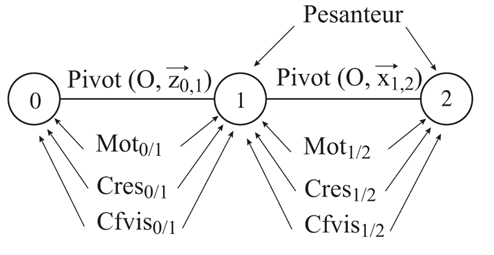
\includegraphics[width=.6\textwidth]{ccs_mp_2017_co_09}

\end{center}
\end{corrige}
\else
\fi


%Q 10 
\question{\label{CCS_MP_2017:q_10}%Répondre à cette question exclusivement sur la figure B du document réponse 
Proposer, en la justifiant, une démarche de résolution permettant d'exprimer, à l'aide de deux équations différentielles en $\varphi$ et $\theta$, les équations de mouvement des solides $\underline{\mathbf{1}}$ et $\underline{\mathbf{2}}$ par rapport au bâti $\underline{\mathbf{0}}$ : il est attendu l'indication de l'ensemble isolé, du théorème utilisé en se limitant strictement au PFD (résultante ou moment avec indication du point d'écriture) et de la direction de projection En utilisant le graphe des liaisons, on ira jusqu'à l'écriture de la projection de l'équation vectorielle (aucun calcul n'est demandé)}
\ifprof
\begin{corrige} ~\\
\begin{center}
\begin{tabular}{lp{5cm}p{7cm}}
\hline
\textbf{Ensemble isolé} & \textbf{Equation scalaire} & \textbf{Justification} \\
\hline
 1 et 2 & 
Théorème du moment dynamique en $O$ en projection sur $\vect{z_{01}}$ 
& On utilise le fait que le moment en (O sur $\vect{z_{01}}$ est nul dans la liaison pivot entre (0) et (1) (les actions mécaniques dans les pivots n’interviendront pas), les actions mécaniques de frottement sec, fluide et du moteur sont connues Nous aurons donc l’équation différentielle souhaitée \\
 2 &	
Théorème du moment dynamique en $O$ en projection sur $\vect{x_{12}}$ 
&On utilise le fait que le moment en ($O$ sur $\vect{x_{12}}$ est nul dans la liaison pivot entre (1) et (2) (les actions mécaniques dans la pivot n’interviendront pas), les actions mécaniques de frottement sec, fluide et du moteur sont connues Nous aurons donc l’équation différentielle souhaitée \\
\hline
\end{tabular}
\end{center}
\end{corrige}
\else
\fi



%Q 11 
\question{\label{CCS_MP_2017:q_11}Mettre en œuvre la démarche explicitée question \ref{CCS_MP_2017:q_10}  et montrer que les équations de mouvement s'écrivent :}
$$ c_{\mathrm{m} 1}+c_{\mathrm{r} 1}=A_{1} \ddot{\varphi}+B_{1} \dot{\varphi}+\frac{\mathrm{d}}{\mathrm{~d} t}\left(\left(C_{11} \sin ^{2} \theta+C_{12} \cos ^{2} \theta\right) \dot{\varphi}\right) 
\quad \text{et} \quad
c_{\mathrm{m} 2}+c_{\mathrm{r} 2}=A_{2} \ddot{\theta}+B_{2} \dot{\theta}+C_{2} \sin (2 \theta) \dot{\varphi}^{2}$$

\textit{où les coefficients constants $A_{1}, B_{1}, C_{11}, C_{12}, A_{2}, B_{2}$ et $C_{2}$ sont à exprimer en fonction de tout ou partie des données de la figure \ref{CCS_MP_2017:fig_10} et de la figure \ref{CCS_MP_2017:fig_11}.}

\ifprof
\begin{corrige}
On isole (1 et 2) et on applique le théorème du moment dynamique en $O$ en projection sur $\vect{z_{01}}$:
$\sum \vectm{O}{\text{ext}}{1+2} \vect{z_{01}}  = \left(\vectmd{O}{1}{0} + \vectmd{O}{2}{0}\right)\cdot \vect{z_{01}}$

On a alors  
$0+0+\dfrac{k_1}{\rho_1} \left(\indice{c}{m1}+\indice{c}{r1}-\indice{f}{Eq1} \varphip \right)=
\deriv{\vectmc{O}{1}{0}\cdot \vect{z_{01}}}{} + \deriv{\vectmc{O}{2}{0}\cdot \vect{z_{01}}}{}$
(car $O$ est centre d’inertie des pièces 1 et 2) Remarque : les deux « 0 » représentent le moment en $O$ sur $\vect{z_{01}}$ de la pesanteur et de la liaison pivot entre 0 et 1

$\vectmc{O}{2}{0} = \inertie{O}{2} \vecto{2}{0} 
= \matinertie{J_{x2}}{J_{y2}}{J_{z2}}{0}{0}{0}{O,\mathcal{B}_2} \begin{pmatrix} \thetap \\ \varphip\sin\theta \\ \varphip \cos \theta \end{pmatrix}_{\mathcal{B}_2}$
$=\begin{pmatrix} J_{x2} \thetap \\ J_{y2}\varphip\sin\theta \\ J_{z2}\varphip \cos \theta \end{pmatrix}_{\mathcal{B}_2}$  (car $O$ est centre d’inertie de 2) De plus $\vz{1}=\begin{pmatrix} 0 \\ \sin\theta \\ \cos \theta \end{pmatrix}_{\mathcal{B}_2}$

$\dfrac{k_1}{\rho_1} \left(\indice{c}{m1}  +\indice{c}{r1}  -\indice{f}{Eq1} \varphip \right)=\indice{J}{z1} \varphipp+\dfrac{\dd \left(\indice{J}{z2} \varphip  \cos^2 \theta+\indice{J}{y2} \varphip \sin^2 \theta\right)}{\dd t}$
  
$\indice{c}{m1}  +\indice{c}{r1}  =\indice{J}{z1}\dfrac{\rho_1}{k_1}\varphipp+\indice{f}{Eq1} \varphip+\dfrac{\dd \left(
\indice{J}{z2}\dfrac{\rho_1}{k_1}\varphip \cos^2 \theta+\indice{J}{y2}\dfrac{\rho_1}{k_1}\varphip \sin^2 \theta \right)}{\dd t}$

Nous obtenons la première équation avec : $A_1=\indice{J}{z1}\dfrac{\rho_1}{k_1}$, $B_1=\indice{f}{Eq1}$, $\indice{C}{11}=\indice{J}{y2}\dfrac{\rho_1}{k_1}$, $\indice{C}{12}=\indice{J}{z2}\dfrac{\rho_1}{k_1}$  

\vspace{1cm}

On isole (2) et on applique le théorème du moment dynamique en ($O$) en projection sur $\vect{x_{1,2}}$

$\sum \vectm{O}{\text{ext}}{2} \vect{x_{1,2}}  = \vectmd{O}{2}{0} \cdot \vect{x_{1,2}} = \deriv{\vectmc{O}{2}{0}\cdot \vect{x_{12}}}{} - \vectmc{O}{2}{0}\cdot\deriv{\vect{x_{12}}}{0}$ (car O est centre d’inertie de la pièce 2)

$0+0+\dfrac{k_2}{\rho_2}\left(\indice{c}{m2}+\indice{c}{r2}-\indice{f}{Eq2}\thetap\right)=\indice{J}{x2}  \thetapp - 
\vectmc{O}{2}{0} \varphip \vy{1}$ (remarque : les deux « 0 » représentent le moment en $O$ sur $\vect{x_{1,2}}$ de la pesanteur et de la liaison pivot entre 1 et 2) De plus $\vy{1}=\begin{pmatrix} 0 \\ \cos\theta \\ \sin \theta \end{pmatrix}_{\mathcal{B}_2}$

$\dfrac{k_2}{\rho_2}\left(\indice{c}{m2}+\indice{c}{r2}-\indice{f}{Eq2}\thetap \right)=\indice{J}{x2} \thetapp-(\indice{J}{y2}-\indice{J}{z2} )   \varphip^2   \sin  \theta  \cos  \theta$

$\indice{c}{m2}+\indice{c}{r2}=\indice{J}{x2}\dfrac{\rho_2}{k_2} \thetapp+\indice{f}{Eq2}\thetap+(\indice{J}{z2}-\indice{J}{y2 })\dfrac{ \rho_2}{2  k_2}\varphip^2   \sin ( 2  \theta)$

Nous obtenons la deuxième équation avec : 
$A_2=\indice{J}{x2}  \dfrac{\rho_2}{k_2}$, $B_2=\indice{f}{Eq2}$ et $C_2=(\indice{J}{z2}-\indice{J}{y2})\dfrac{\rho_2}{2 k_2}$

\end{corrige}
\else
\fi



%IVC4) 
\subsubsection{Identification des éléments cinétiques équivalents}
\ifprof
\else
La complexité des formes des pièces et de la structure géométrique ainsi que la présence de nombreux guidages impliquent une grande difficulté de détermination de l'inertie, du frottement visqueux et du couple résistant équivalents rapportés à l'axe moteur à partir du seul modèle de connaissance : il est donc nécessaire de procéder à une identification comportementale en charge des deux axes afin d'évaluer ces grandeurs.\\
Afin de simplifier l'étude, l'identification des paramètres du modèle décrivant la dynamique des deux chaines va s'effectuer de façon découplée : les moteurs sont donc alimentés alternativement et on suppose par ailleurs que le bloc optique est positionné horizontalement, soit $\theta=0^{\circ}$, pour l'étude de l'axe d'azimut seul.\\
\fi
%Q 12 
\question{\label{CCS_MP_2017:q_12}Dans le cadre de ces configurations découplées, simplifier les équations de la question \ref{CCS_MP_2017:q_11}.  Donner les expressions des moments d'inertie équivalents $J_{\mathrm{Eq} \varphi}$ et $J_{\mathrm{Eq} \theta}$ respectivement par rapport aux axes d'azimut et d'élévation, en fonction des coefficients constants $A_{i}, B_{i}$ et $C_{i}$. Donner alors les expressions des moments d'inerties équivalents $J_{\mathrm{Eq} 1}$ et $J_{\mathrm{Eq} 2}$ au niveau des arbres moteurs des deux machines à courant continu en fonction de ces mêmes coefficients et de tout ou partie des données de la figure \ref{CCS_MP_2017:fig_11}.}
\ifprof
\begin{corrige}
Dans le cas particulier où $\theta=0\degres$, nous obtenons :
$\indice{c}{m1} +\indice{c}{r1} =A_1 \varphipp +B_1 \varphip + C_{12} \varphipp$   et  $\indice{c}{m2}+\indice{c}{r2}=A_2 \thetapp + B_2 \thetap$.

Nous pouvons donc définir : $J_{\text{eq} \varphi}=A_1  +C_{12}$ et $J_{\text{eq} \theta}=A_2$ .

Pour ramener ces moments d’inertie sur les axes des moteurs, il faut « égaler les énergies cinétiques » :
$\dfrac{1}{2} {J}_{eq\varphi} \varphip^2 = \dfrac{1}{2}\indice{J}{Eq1}\indice{\omega}{m1}^2$
$\Rightarrow \indice{J}{Eq1} = {J}_{eq\varphi}\dfrac{\varphip^2}{\indice{\omega}{m1}^2} \rho_1^2$

$\Rightarrow   \indice{J}{Eq1} = {J}_{eq\varphi} \rho_1^2=(A_1  +C_{12} )\rho_1^2$
De la même façon, $\indice{J}{Eq2} ={J}_{\text{eq} \theta}\rho_2^2 =A_2 \rho_2^2$


\end{corrige}
\else
\fi

\ifprof
\else
Le comportement d'une machine à courant continu utilisée en moteur est décrit par les équations de la figure \ref{CCS_MP_2017:fig_12}.

\begin{figure}[!h]
\centering
\begin{tabular}{p{8cm}p{6cm}}
\hline
Théorème d'obtention de l'équation & Équation différentielle \\
\hline
Loi des mailles appliquée au modèle électrique équivalent  & $u_{\mathrm{mi}}(t)=R i_{\mathrm{i}}(t)+L \dfrac{\mathrm{~d} i_{\mathrm{i}}(t)}{\mathrm{d} t}+e_{\mathrm{i}}(t)$ \\

Théorème de l'énergie cinétique appliqué à l'ensemble mécanique entrainé par la machine à courant continu
 & 
 $J_{\mathrm{Eq} i} \dfrac{\mathrm{~d} \omega_{\mathrm{mi}}(t)}{\mathrm{d} t}=c_{\mathrm{mi}}(t)+c_{\mathrm{ri}}(t)-f_{\mathrm{Eqi}} \omega_{\mathrm{mi}}(t)$ \\

Équations de couplage électro-mécanique dans l'induit de la machine à courant continu & 
$c_{\mathrm{mi}}(t)=K_{\mathrm{T}} i_{\mathrm{i}}(t) \quad$ et $\quad e_{\mathrm{i}}(t)=K_{\mathrm{E}} \omega_{\mathrm{mi}}(t)$ \\
$\mathrm{avec} K_{\mathrm{T}}=K_{\mathrm{E}}=K$  \\
\hline
\end{tabular}

%Figure 12 
\caption{Équations de modélisation du comportement d'une machine à courant continu \label{CCS_MP_2017:fig_12}}

\end{figure}
La machine à courant continu Faulhaber 2224-U006-SR utilisée pour la motorisation des deux axes d'azimut et 
d'élévation a les caractéristiques suivantes:

\begin{itemize}
  \item tension nominale $U_{0}=\SI{6}{V}$;
  \item résistance $R=1,94\,\Omega$ et inductance d'induit $L=45 \mu \mathrm{H}$;
  \item constante de couplage $K=K_{\mathrm{T}}=K_{\mathrm{E}}$ avec $K_{T}=6,92 \times 10^{-3} \mathrm{~N} \cdot \mathrm{~m} \cdot \mathrm{~A}^{-1}$ et $K_{E}=6,92 \times 10^{-3} \mathrm{~V} \cdot \mathrm{~s} \cdot \mathrm{rad}{ }^{-1}$
\end{itemize}

Par ailleurs, pour chacun des axes (axe d'azimut, indice 1, et axe d'élévation, indice 2) :

\begin{itemize}
  \item $J_{\text {Eqi }}\left(\mathrm{en} \mathrm{kg} \cdot \mathrm{m}^{2}\right)$ et $f_{\text {Eqi }}\left(\mathrm{en} \mathrm{N} \cdot \mathrm{m} \cdot \mathrm{s} \cdot \mathrm{rad}^{-1}\right)$ sont respectivement l'inertie et le coefficient de frottement visqueux équivalents rapportés à l'axe de rotation de la machine à courant continu de l'axe $i$;
  \item $u_{\mathrm{mi}}(t)(\mathrm{en} \mathrm{V}), i_{\mathrm{i}}(t)$ (en A$)$ et $e_{\mathrm{i}}(t)$ (en V$)$ sont respectivement la tension d'alimentation, l'intensité dans l'induit et la force contre-électromotrice de la machine à courant continu de l'axe $i$;
  \item $\omega_{\mathrm{mi}}(t)\left(\mathrm{en} \mathrm{rad} \cdot \mathrm{s}^{-1}\right)$ est la vitesse de rotation de la machine à courant continu de l'axe $i$.
\end{itemize}

Les transformées de Laplace des fonctions temporelles seront notées en majuscule : ainsi, pour la vitesse angulaire du moteur, on notera $\Omega_{\mathrm{mi}}(p)=\mathcal{L}\left[\omega_{\mathrm{mi}}(t)\right]$ où $\mathcal{L}$ est l'opérateur et $p$ la variable symbolique de Laplace.\\
Dans toute la suite du problème, les conditions initiales de Heaviside sont supposées être vérifiées.\\
\fi
%Q 13 
\question{\label{CCS_MP_2017:q_13}Répondre à cette question exclusivement sur la figure C du document réponse. Compléter la partie correspondant au schéma-bloc associé à la machine à courant continu de l'axe d'azimut dont le fonctionnement est décrit par les équations données figure \ref{CCS_MP_2017:fig_12}. Compléter également le dernier bloc vide de ce schéma d'asservissement.}
\ifprof
\begin{corrige}
\end{corrige}
\else
\fi


%IVC5) 
\subsubsection{Identification des constantes de la machine à courant continu de l'axe d'azimut en charge}
\ifprof
\else
Afin d'identifier les valeurs de ses constantes en charge, des essais ont été réalisés sur la machine à courant continu assurant la motorisation de l'axe d'azimut : pour ces essais, le bloc optique $\underline{\mathbf{2}}$ a été placé horizontalement (angle $\theta=0^{\circ}$ ), ce qui correspond à la configuration la plus contraignante au niveau du comportement dynamique.\\
Pour réaliser l'identification des paramètres équivalents, la machine à courant continu est alimentée par une tension suivant une loi en échelon d'amplitude $u_{0}$ connue: le courant $i_{1}(t)$ dans l'induit est alors mesuré par une pince ampèremétrique et son évolution est affichée sur un oscilloscope. La figure D du document réponse regroupe les copies d'écran de trois mesures à différentes tensions ainsi qu'un zoom de la troisième mesure.\\
\fi

%Q 14 
\question{\label{CCS_MP_2017:q_14}À partir de l'analyse des comportements en régime permanent, justifier que le frottement visqueux équivalent (coefficient $f_{E q 1}$ ) au niveau de l'axe d'azimut a une influence négligeable et que le couple résistant équivalent $c_{r 1}$ peut être considéré comme constant Estimer la valeur $c_{\mathrm{r} 10}$ de ce couple résistant.}
\ifprof
\begin{corrige}
La figure D du document réponse montre que, en régime établi, « l’intensité finale » est voisine de \SI{0,2}{A} et ce pour les tensions de \SI{4,9}{V}, \SI{5,9}{V} et \SI{6,9}{V}
Avec l’équation $\indice{c}{m1}  (t)=K  i(t)$, nous savons que le couple moteur est proportionel à l’intensité. Cela signifie que, en régime établi, le couple moteur ne dépend pas de la tension d’alimentation (donc de la vitesse de rotation du système) puisque l’intensité finale est toujours la même.
En régime établi, le couple moteur compense les frottements sec et visqueux. Comme ce couple moteur est constant pour la gamme de tension (donc de vitesse) testée, cela signifie que les frottementsvisqueux (qui dépendent de la vitesse) ne sont pas prépondérants par rapport au frottement sec.
Il est donc possible d’affirmer que le frottement visqueux équivalent a une influence négligeable (par rapport au couple de frottement sec).
\subparagraph*{Estimation du couple résistant}
Les frottements visqueux étant négligeables, les équations précédentes donnent en régime permanent :
$\indice{C}{r1}(t)=-\indice{C}{m1}(t)=-K i(t)$ 

A N :  $\indice{C}{r1}(t)=-6,92\times 1^{-3} \times  0,2 = -\SI{1,4e-3}{Nm}$ $\Rightarrow   
\indice{C}{r1} (t)=-\SI{1,4 e-3}{Nm}$  

\end{corrige}
\else
\fi

\ifprof
\else
Sur les courbes de mesure, la montée initiale de courant est quasi instantanée, ce qui est révélateur d'une influence faible de l'inductance $L$ et, par ailleurs, la question précédente a mis en évidence l'influence négligeable du frottement visqueux équivalent : par conséquent, dans la suite, on néglige ces termes, soit $L=0$ et $f_{\mathrm{Eq} 1}=0$ On donne les deux transformées inverses suivantes : $\dfrac{1}{\alpha p+\beta} \xrightarrow{\mathcal{L}^{-1}} \dfrac{1}{\alpha} \mathrm{e}^{-\dfrac{\beta}{\alpha} t}$ et $\dfrac{1}{p(\alpha p+\beta)} \xrightarrow{\mathcal{L}^{-1}} \dfrac{1}{\beta}\left(1-\mathrm{e}^{-\dfrac{\beta}{\alpha} t}\right)$ et, pour les calculs, il est possible de poser $T_{1}=\alpha / \beta$.
\fi

%Q 15 
\question{\label{CCS_MP_2017:q_15}Montrer que, dans le cadre des simplifications précédentes et dans le cas d'un échelon de tension d'alimentation d'amplitude $u_{0}, I_{1}(p)=\dfrac{1}{K^{2}+R J_{\mathrm{Eq} 1} p}\left(J_{\mathrm{Eq} 1} u_{0}-K \dfrac{c_{\mathrm{r} 10}}{p}\right)$. En déduire l'expression temporelle de l'intensité $i_{1}(t)$ en utilisant les transformées symboliques inverses fournies précédemment.}
\ifprof
\begin{corrige}
En écrivant ce que l’on voit sur le schémabloc de la figure C, nous obtenons la relation :
$\{(\indice{U}{m1}  (p)-K  \indice{\Omega}{m1}  (p)) \dfrac{K}{R}+\indice{C}{r1} (p)\}  \dfrac{1}{\indice{J}{eq1}  p}=\indice{\Omega}{m1} (p)$

$\indice{U}{m1}  (p)   \dfrac{K}{(R  \indice{J}{eq1}   p}+\indice{C}{r1} (p) \dfrac{1}{\indice{J}{eq1} p}=\indice{\Omega}{m1} (p) \left\{1+\dfrac{K^2}{R \indice{J}{eq1}  p}\right\}$

$\indice{U}{m1}  (p)  \dfrac{K}{(^2+R \indice{J}{eq1}   p}+\indice{C}{r1} (p)   \dfrac{R}{K^2+R  \indice{J}{eq1}  p}=\indice{\Omega}{m1} (p)$
    Avec $(\indice{U}{m1}  (p)-K  \indice{\Omega}{m1}  (p))  \dfrac{1}{R}=I_1 (p)$

Nous obtenons : 
$\indice{U}{m1}  (p) \dfrac{K}{K^2+R  \indice{J}{eq1}  p}+\indice{C}{r1} (p)\dfrac{R}{K^2+R \indice{J}{eq1}  p}=\indice{\Omega}{m1} (p)=\dfrac{\indice{U}{m1}  (p)-R I_1 (p)}{K}$

$\indice{U}{m1}  (p)  \left(\dfrac{K^2}{K^2+R  \indice{J}{eq1}   p }-1\right)+\indice{C}{r1} (p) \dfrac{KR}{K^2+R \indice{J}{eq1}  p}=-R  I_1 (p)$

$I_1 (p)=\indice{U}{m1}  (p) \left( \dfrac{\indice{J}{eq1}p}{K^2+R  \indice{J}{eq1}  p}\right)-\indice{C}{r1} (p) \dfrac{K}{K^2+R \indice{J}{eq1}p}$

$I_1 (p)=\dfrac{1}{K^2+R \indice{J}{eq1}  p} \left[\indice{U}{m1}  (p)  \indice{J}{eq1}  p-\indice{C}{r1} (p) K\right]$

Pour des entrées échelons, l’expression devient : $I_1 (p)=\dfrac{1}{K^2+R \indice{J}{eq1}  p}  \left[u_0  \indice{J}{eq1}-\dfrac{\indice{C}{r10}}{p}  K\right]$

Par transformée de Laplace inverse, l’intensité, dans le domaine temporel, s’écrit :
$i_1 (t)=\dfrac{u_0  \indice{J}{eq1}}{R  \indice{J}{eq1} } \text{e}^{-t  \dfrac{K^2}{R  \indice{J}{eq1} }}-\dfrac{\indice{C}{r10}  K}{K^2}    \left(1-\text{e}^{-t  \dfrac{K^2}{R  \indice{J}{eq1}}} \right)$

$i_1 (t)=\dfrac{u_0}{R} \text{e}^{-t \dfrac{K^2}{R  \indice{J}{eq1}}}-\dfrac{\indice{C}{r10}}{K}   \left(1- \text{e}^{-t\dfrac{K^2}{R  \indice{J}{eq1} }}\right)$
$=\dfrac{u_0}{R}  \text{e}^{-\dfrac{t}{T_1}}-\dfrac{\indice{C}{r10}}{K}  \left(1- \text{e}^{-t /T_1}\right )$

%
%
\end{corrige}
\else
\fi


%Q 16 
\question{\label{CCS_MP_2017:q_16}En indiquant la méthode employée, estimer la valeur de la constante de temps $T_{1}$ associée à l'axe d'azimut dans cette configuration contraignante (laisser les traits de construction sur la figure D du document réponse) En déduire la valeur estimée de l'inertie équivalente $J_{\mathrm{Eq1}}$ rapportée à l'arbre moteur de l'axe d'azimut dans le cas où le bloc optique $\underline{2}$ est placé en position horizontale}
\ifprof
\begin{corrige}
On a $\dfrac{\dd i_1 (t)}{\dd t}=\dfrac{-1}{T_1} \left[\dfrac{u_0}{R}+\dfrac{\indice{C}{r10}}{K}\right]\text{e}^{-t /T_1}$

A $t = 0+$, la pente de la courbe d’intensité est : $\dfrac{\dd i_1 (t=0+)}{\dd t}=-\dfrac{1}{T_1}  \left[ \dfrac{u_0}{R}+\dfrac{\indice{C}{r10}}{K}\right]$

Avec $i_1(t=0+)=\dfrac{u_0}{R}$ et $i_1(t\to +\infty)= - \dfrac{\indice{C}{r10}}{K}$, cela signifie que la tangente à l’origine coupe la valeur asymptotique pour $t=T_1$

Le zoom de la figure D, permet de mesurer $T_1 \simeq \SI{22}{ms}$

Avec $T_1=\dfrac{R\indice{J}{eq1}}{K^2}$, $\indice{J}{eq1} =\dfrac{K^2  T_1}{R}$


AN :  $\indice{J}{eq1} =\dfrac{\left(6,92\times 10^{-3} \right)^2 \times  22 \times 10^{-3}}{1,94} =5,43 \times 10 ^{-7} \si{kgm^2}$

\end{corrige}
\else
\fi


%IVC6)
\subsubsection{ Modulation de la tension électrique d'alimentation de la machine à courant continu}
\ifprof
\else
La modulation de la tension électrique pour l'alimentation des machines à courant continu associées aux deux chaines est réalisée par des hacheurs à commande numérique à deux quadrants réversibles en tension.\\
Le hacheur est un convertisseur statique qui permet d'alimenter la machine à courant continu dans les deux sens en gérant précisément la tension d'alimentation : la modulation de la tension électrique d'amplitude $U_{0}=6 \mathrm{~V}$ (tension nominale des moteurs) est réalisée de la façon présentée figure \ref{CCS_MP_2017:fig_13}.\\

\begin{figure}[!h]
\centering
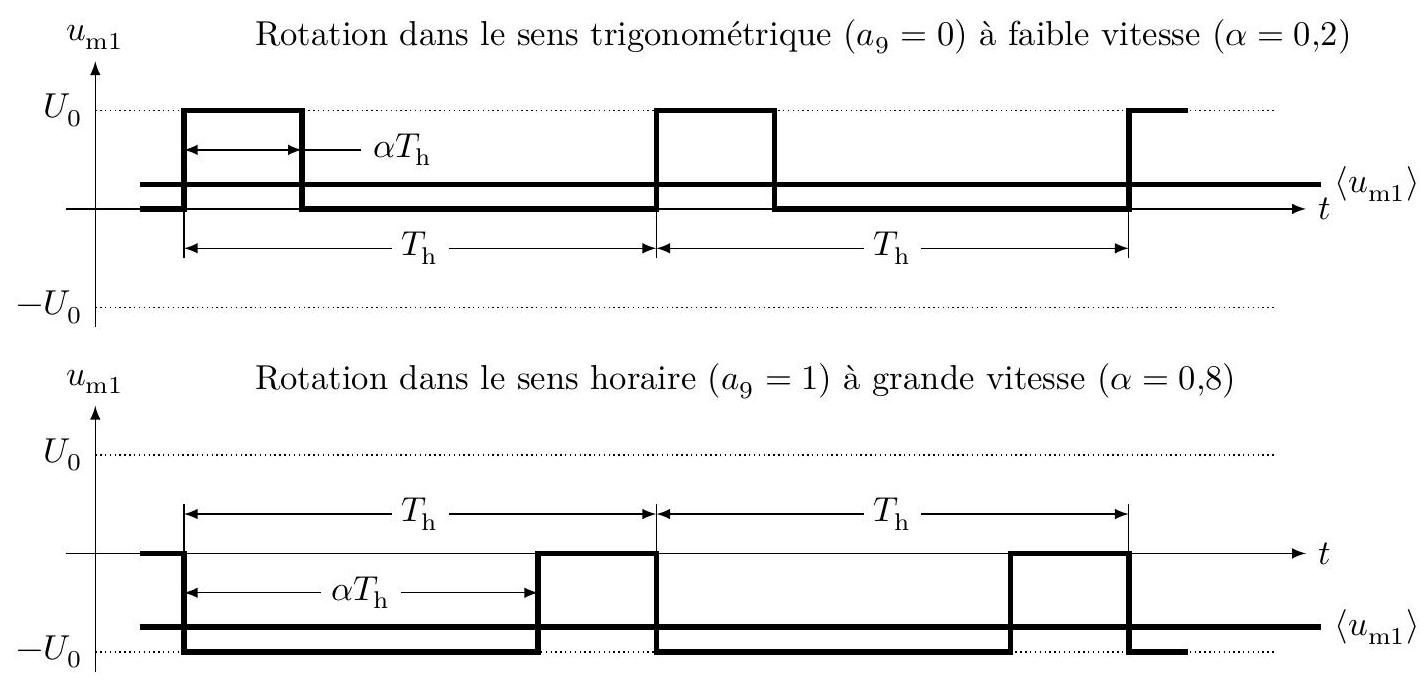
\includegraphics[width=\textwidth]{2024_12_07_51b7f57c7f055c2d8d29g-09}

%Figure 13 
\caption{Tension hachée délivrée par le hacheur à la machine à courant continu : le signe de la tension et la valeur du rapport cyclique $0 \leqslant \alpha \leqslant 1$ sont définis par le mot binaire envoyé \label{CCS_MP_2017:fig_13}}
\end{figure}

Dans la station totale Leica tcra 1103, la fréquence de hachage est d'environ $f_{\mathrm{h}}=20 \mathrm{kHz}$, ce qui correspond à une période de séquence $T_{\mathrm{h}}=50 \mu \mathrm{~s}$, très inférieure à la constante de temps identifiée question \ref{CCS_MP_2017:q_16}  : seule la valeur moyenne $\left\langle u_{\mathrm{m} 1}\right\rangle$ est donc ressentie par la machine à courant continu.\\
Le pilotage du hacheur se fait par l'envoi, par la carte de commande selon une liaison série, d'un mot binaire de 10 bits noté $a_{9} a_{8} a_{7} a_{6} a_{5} a_{4} a_{3} a_{2} a_{1} a_{0}$ Le bit $a_{9}$ définit le signe avec, par choix, $a_{9}=0$ pour une rotation de l'arbre moteur dans le sens trigonométrique et $a_{9}=1$ pour une rotation dans le sens horaire Les 9 bits suivants $a_{8}$ à $a_{0}$ permettent de définir la valeur du rapport cyclique $\alpha$ (figure \ref{CCS_MP_2017:fig_13}):
\begin{itemize}
  \item le rapport cyclique $\alpha=0$ quand $a_{8} a_{7} a_{6} a_{5} a_{4} a_{3} a_{2} a_{1} a_{0}=000000000$ et, dans ce cas, le moteur ne tourne pas car la tension moyenne envoyée $\left\langle u_{\mathrm{m} 1}\right\rangle=0 \mathrm{~V}$;
  \item le rapport cyclique $\alpha=1$ quand $a_{8} a_{7} a_{6} a_{5} a_{4} a_{3} a_{2} a_{1} a_{0}=111111111$ et, dans ce cas, le moteur tourne à sa vitesse maximale car la tension moyenne envoyée est $\left\langle u_{\mathrm{m} 1}\right\rangle= \pm U_{0}$ selon le signe défini par la variable $a_{9}$;
  \item les combinaisons intermédiaires de $a_{0}$ à $a_{8}$ permettent de définir la valeur du rapport cyclique $\alpha$.
\end{itemize}
\fi

%Q 17 
\question{\label{CCS_MP_2017:q_17}On suppose que le comportement du hacheur est linéaire en fonction du rapport cyclique $\alpha$ : calculer la valeur du gain linéarisé $K_{\mathrm{h} 1}$ du hacheur, en $\mathrm{V} \cdot$ points ${ }^{-1}$, où les points correspondent à la valeur du nombre entier codé par le mot binaire $a_{8} a_{7} a_{6} a_{5} a_{4} a_{3} a_{2} a_{1} a_{0}$}
\ifprof
\begin{corrige}
Le hacheur est modélisable (avec les hypothèses du sujet) par un système proportionnel dont le gain s’écrit : 
$\indice{K}{h1} = \dfrac{U_0}{2^9-1}$
 AN : $\indice{K}{h1} =1,17 \times 10^{-2}\si{V/point}$
\end{corrige}
\else
\fi



%IVC7) 
\subsubsection{Réglage du gain de l'adaptateur}
\ifprof
\else
Les exigences associées à la mesure de distances variant en continu imposent la conception de lois de commande dédiées aux asservissements en position des deux axes. Ces lois permettent, d'une part, de suivre le déplacement dans le plan azimutal du prisme optique rétro-réfléchissant en s'adaptant aux variations de vitesse de l'opérateur et, d'autre part, de compenser les variations d'altitude inhérentes au profil du sol.\\
Dans le cas de l'axe d'azimut, l'adaptateur situé entre l'entrée et le comparateur a un comportement assimilable à un gain pur $K_{\mathrm{ad} 1}$ (figure C du document réponse) Le réglage de sa valeur permet d'assurer un écart en sortie du comparateur $\varepsilon_{1}=0$ lorsque l'erreur de positionnement en azimut par rapport à la consigne $\zeta=\varphi_{\mathrm{c}}-\varphi=0$.\\
\fi

%Q 18 
\question{\label{CCS_MP_2017:q_18}Justifier que $K_{\mathrm{ad} 1}=K_{\mathrm{c} 1} / \rho_{1}$ Donner sa valeur numérique et préciser son unité.}

\ifprof
\begin{corrige}
Les blocs Adaptateur, Codeur incrémental et Réducteurs sont modélisés par des systèmes proportionnels, il est donc possible d’écrire la relation temporelle :  $\varepsilon_1 (t)=\varphi_c (t)  \indice{K}{ad1}-\dfrac{\indice{K}{c1}}{\rho_1} \varphi (t)$
Pour obtenir $\varepsilon_1  (t_{\infty})=0$ lorsque $\varphi_c (t_{\infty})=\varphi(t_{\infty})$ , il faut $\indice{K}{ad1}=\dfrac{\indice{K}{c1}}{\rho_1}$ 

\end{corrige}
\else
\fi

%
\subsubsection{ Synthèse de la loi de commande dédiée à la chaine d'azimut}
\ifprof
\else
Le moment d'inertie équivalent $J_{E q 1}$ est considéré constant et égal à sa valeur maximale, obtenue lorsque le bloc optique $\underline{\mathbf{2}}$ est en position horizontale (angle d'élévation $\theta=0^{\circ}$ ), tel que déterminé question \ref{CCS_MP_2017:q_16}.\\
Afin de simplifier l'étude proposée, le déplacement du prisme optique rétro-réfléchissant par rapport au sol sera considéré comme horizontal dans la suite : dans ce cas, la chaine d'élévation (angle $\theta$ ) n'est pas sollicitée.

La phase de modélisation a permis de construire un modèle de connaissance sous forme du schéma-bloc fourni figure C du document réponse. Suite aux conclusions sur l'identification réalisée précédemment sur le moteur en charge, les versions simplifiées des fonctions de transfert obtenues question \ref{CCS_MP_2017:q_13} associées au modèle linéarisé de la machine à courant continu sont $M_{1}(p) \simeq \frac{K}{K^{2}+R J_{\text {Eq1 }} p}$ et $G_{1}(p) \simeq \frac{R}{K^{2}+R J_{\text {Eq1 }} p}$.
Un correcteur à action proportionnelle de gain $C_{1}(p)=K_{\mathrm{p} 1}>0$ est tout d'abord choisi.
\fi

%Q 19 
\question{\label{CCS_MP_2017:q_19}Donner les expressions, en fonction du gain $K_{\mathrm{p} 1}$ et des données du schéma-bloc de l'asservissement de l'axe d'azimut présenté sur la figure C du document réponse, des coefficients $K_{1 \mathrm{r}}, a_{1}$ et $a_{2}$ tels que}

$$
\Phi(p)=\frac{\Phi_{\mathrm{c}}(p)+K_{1 \mathrm{r}} C_{\mathrm{r} 1}(p)}{1+a_{1} p+a_{2} p^{2}}
$$

\textit{Justifier que l'asservissement étudié reste stable pour toute valeur de $K_{\mathrm{p} 1}>0$}

\ifprof
\begin{corrige}
Sur la figure C, nous « lisons » :
$\left\{(\Phi_c (p)  \indice{K}{ad1} -\dfrac{\indice{K}{c1} }{\rho_1 }  \Phi (p))   \dfrac{\indice{K}{p1} \indice{K}{h1}   K }{K^2+R  \indice{J}{Eq1}   p }+\indice{C}{r1}  (p)R/(K^2+R  \indice{J}{Eq1}   p )\right\}   \rho_1/p=\Phi(p)$

En regroupant et en utilisant la relation de la question précédente

$\Phi_c (p)   \dfrac{\indice{K}{ad1}   K _p1    \indice{K}{h1}  K  \rho_1}{\left(K^2+R  \indice{J}{Eq1}   p \right) p} +\indice{C}{r1}(p) \dfrac{R  \rho_1}{\left(K^2+R  \indice{J}{Eq1}   p \right) p} 
=\Phi(p)\left(1+\dfrac{\indice{K}{ad1}   K _p1    \indice{K}{h1}  K  \rho_1}{\left(K^2+R  \indice{J}{Eq1}   p \right) p} \right)$

$\Phi(p)=\dfrac{\Phi_c (p)  \indice{K}{ad1}   K _p1    \indice{K}{h1}  K  \rho_1+\indice{C}{r1}  (p) R  \rho_1}{\indice{K}{ad1}   \indice{K}{p1}    \indice{K}{h1}  K  \rho_1+K^2 p +R  \indice{J}{Eq1}    p ^2 }$

$\Phi(p)=  \dfrac{\Phi_c (p)+\indice{C}{r1}  (p)   \dfrac{R  \rho_1}{\indice{K}{ad1}   K _p1    \indice{K}{h1}  K  \rho_1 }}{1+\dfrac{K^2}{\indice{K}{ad1}   K _p1    \indice{K}{h1}  K  \rho_1 } p +\dfrac{R  \indice{J}{Eq1} }{\indice{K}{ad1}   K _p1    \indice{K}{h1}  K  \rho_1 }   p ^2 }$
 
Nous obtenons : $\indice{K}{1r}=  \dfrac{R  \rho_1}{\indice{K}{ad1}   K _p1    \indice{K}{h1}  K  \rho_1 }$ ; 
$a_1=  \dfrac{K^2}{\indice{K}{ad1}   \indice{K}{p1}    \indice{K}{h1}  K  \rho_1}$ ; 
$b_1=  \dfrac{R  \indice{J}{Eq1} }{\indice{K}{ad1}   \indice{K}{p1}    \indice{K}{h1}  K  \rho_1 }$

En utilisant $\indice{K}{c1}$   à la place de $\indice{K}{ad1}$, nous obtenons : 
$\Phi(p)=  \dfrac{\Phi_c (p)+\indice{C}{r1}  (p)   \dfrac{R  \rho_1}{\indice{K}{c1}   K _p1    \indice{K}{h1}  K }}{1+\dfrac{K}{\indice{K}{c1}   K _p1    \indice{K}{h1}  } p +\dfrac{R  \indice{J}{Eq1} }{\indice{K}{c1}   K _p1    \indice{K}{h1}  K }   p ^2 }$ ;

$\indice{K}{1r}=  \dfrac{R  \rho_1}{\indice{K}{c1}   K _p1    \indice{K}{h1}  K }$; 
$a_1=  \dfrac{K}{\indice{K}{c1}   K _p1    \indice{K}{h1} }$ ; 
$b_1=  \dfrac{R  \indice{J}{Eq1} }{\indice{K}{c1}   K _p1    \indice{K}{h1}  K }$

La fonction de transfert globale du schémabloc de la figure C est du second ordre. Un système de second ordre est inconditionnellement stable si tous les coefficients du dénominateur sont strictement positifs Les coefficients $a_1$, $b_1$, $\indice{K}{1r}$ sont strictement positifs si $\indice{K}{p1}$  est lui-même strictement positif (les autres coefficients intervenant dans ces expressions sont strictement positifs)

\end{corrige}
\else
\fi

\ifprof
\else
Afin de permettre un suivi en continu du prisme optique rétro-réfléchissant et un recalage de la ligne de visée sur son centre avant la mesure, il est nécessaire d'implanter un correcteur pouvant garantir une erreur de positionnement angulaire $\Delta \varphi \leqslant 1 \times 10^{-4} \mathrm{rad}$ pour une distance de mesure $D=500 \mathrm{~m}$.\\
\fi

%Q 20 
\question{\label{CCS_MP_2017:q_20}Déterminer l'expression, en fonction des coefficients $K_{1 r}, a_{1}$ et
 $a_{2}$ établis question \ref{CCS_MP_2017:q_19} , de l'erreur en azimut $\zeta(p)=\Phi_{c}(p)-\Phi(p)$ lorsque
 la consigne angulaire est une rampe de pente $\Omega_{\mathrm{c} 0}$ 
 (soit $\Phi_{\mathrm{c}}(p)=\Omega_{\mathrm{c} 0} / p^{2}$ ) 
 et le couple résistant est un échelon d'amplitude 
 $c_{\mathrm{r} 10}$ (soit $ C_{\mathrm{r} 1}(p)= \dfrac{c_{\mathrm{r} 10}}{p}$).}
\ifprof
\begin{corrige}
$\xi(p)=\Phi_c (p)-\Phi(p)=\Phi_c (p)  \left[1- \dfrac{1}{1+a_1 p +b_1   p ^2 }\right]-\dfrac{\indice{K}{1r}}{1+a_1 p +b_1   p ^2 }   \indice{C}{r1} (p)$

$\xi(p)=\Phi_c (p)   \dfrac{p  \left(a_1+b_1  p \right)}{1+a_1 p +b_1   p ^2 }-\dfrac{\indice{K}{1r}}{1+a_1 p +b_1   p ^2 }   \indice{C}{r1} (p)$

Pour les signaux donnés : $\xi(p)=\dfrac{\Omega_{\text{c0}}}{p^2}     \dfrac{p  (a_1+b_1  p )}{1+a_1 p +b_1   p ^2 }-\dfrac{\indice{K}{1r}}{1+a_1 p +b_1   p ^2 } \dfrac{\indice{C}{r10}}{p}$.

\end{corrige}
\else
\fi


%Q 21 
\question{\label{CCS_MP_2017:q_21}Établir l'expression du gain minimal $K_{\mathrm{p} 1}$ permettant la réalisation d'une mesure en continu en fonction de tout ou partie des paramètres de la figure C du document réponse Donner sa valeur numérique pour une pente de position $\Omega_{\mathrm{c} 0}=V_{\mathrm{Max}} / D \approx 2,78 \times 10^{-3} \mathrm{rad} \cdot \mathrm{s}^{-1}$ et un couple résistant $c_{\mathrm{r} 10} \approx-1,3 \times 10^{-3} \mathrm{~N} \cdot \mathrm{~m}$}
\ifprof
\begin{corrige}
Le système étudié (sa modélisation) étant stable, il est possible d’appliquer le théorème de la valeur finale : 
$\Delta \varphi=
\lim\limits_{t\to+\infty)}\xi (t)
=\lim\limits_{p\to 0}p\xi(p)
=\lim\limits_{p\to0} p  \left( 
\dfrac{\Omega_{\text{c0}}}{p^2}
\dfrac{p(a_1+b_1p)}{1+a_1 p +b_1   p ^2 }
-\dfrac{\indice{K}{1r}}{1+a_1 p +b_1   p ^2 }   
\dfrac{\indice{C}{r10}}{p} \right)$

$\Delta \varphi
=a_1  \Omega_{\text{c0}} -\indice{K}{1r}   \indice{C}{r1}0
=  (K^2   \Omega_{\text{c0}} -R  \rho_1   \indice{C}{r1}0)/(\indice{K}{ad1}   K _p1    \indice{K}{h1}  K  \rho_1 )$

Soit : 
$\indice{K}{p1} = \dfrac{K^2   \Omega_{\text{c0}} -R  \rho_1   \indice{C}{r10}}{\Delta \varphi  \indice{K}{ad1}   \indice{K}{h1}  K  \rho_1 } \quad    \indice{K}{p1 mini} = \dfrac{K^2   \Omega_{\text{c0}} -R  \rho_1   \indice{C}{r1}0}{\Delta \varphi_{\text{Maxi}}   \indice{K}{ad1}   \indice{K}{h1}  K  \rho_1 }$

AN  $\indice{K}{p1 mini } = \dfrac{(6,92  10^{-3} )^2   2,78  10^{-3}+1,94   2/7 210    1,3  10^{-3}}{1  10^{-4}    81,49 /(2/7 210 ) 1,17   6 ,92  10^{-3}    2/7 210 }=5,4  10^{-2}$.

\end{corrige}
\else
\fi

\ifprof
\else
La synthèse de ce correcteur doit garantir une marge de phase $M_{\mathrm{Ph}}=45^{\circ}$ à la pulsation $\omega_{1}=2 \times 10^{4} \mathrm{rad} \cdot \mathrm{s}^{-1}$ (ces valeurs sont obtenues suite à une étude non proposée dans le cadre de ce sujet).\\
Le tracé, dans le plan de BODE, de la réponse fréquentielle de la fonction de transfert en boucle ouverte de l'asservissement de l'axe d'azimut pour une correction unitaire (gain $K_{\mathrm{p} 1}=1$, grandeur sans unité) est fournie, en trait continu fort, figure E du document réponse.\\
\fi

%Q 22 
\question{\label{CCS_MP_2017:q_22}
%Répondre à cette question exclusivement sur la figure E du document réponse 
Un correcteur à action proportionnelle permet-il de respecter les spécifications du cahier des charges (commenter les constructions sur le graphe et dans la zone prévue à cet effet) ?}
\ifprof
\begin{corrige}
Un correcteur proportionnel ne modifie pas la courbe de phase du diagramme de Bode Or à $\omega_1=2\times 10^4 \si{rad/s}$  la phase de la FTBO non corrigée (donc également pour la FTBO corrigée avec un correcteur proportionnel) vaut sensiblement $-180\degres$. Il n’est donc pas possible d’avoir une phase de $-135\degres$ à cette pulsation qui pourrait assurer la marge de phase souhaitée
Un correcteur proportionnel ne permet pas de satisfaire le critère de marge de phase

\end{corrige}
\else
\fi

%
%Afin de répondre aux exigences du cahier des charges en terme de marge de phase, un correcteur à avance de phase de fonction de transfert $C_{1}(p)=K_{\mathrm{p} 1} \frac{1+a T_{\mathrm{d}} p}{1+T_{\mathrm{d}} p}$ est choisi : dans cette fonction de transfert, $K_{\mathrm{p} 1}>0$ est un gain sans unité, $a>1$ est un facteur sans unité et $T_{\mathrm{d}}>0$ est une constante de temps en seconde\\
%
%%Q 23 
%\question{\label{CCS_MP_2017:q_23}Après avoir déterminé la valeur de la phase $\varphi_{\mathrm{m}}$ que le correcteur à avance de phase doit apporter à la pulsation $\omega_{1}=2 \times 10^{4} \mathrm{rad} \cdot \mathrm{s}^{-1}$ pour imposer la marge de phase $M_{\mathrm{Ph}}=45^{\circ}$ souhaitée, déterminer les valeurs numériques du facteur $a$ et de la constante de temps $T_{\mathrm{d}}$ sachant que $a=\frac{1+\sin \varphi_{\mathrm{m}}}{1-\sin \varphi_{\mathrm{m}}}$ et $\omega_{1}=\frac{1}{T_{\mathrm{d}} \sqrt{a}}$}
%\ifprof
%\begin{corrige}
%\end{corrige}
%\else
%\fi
%
%
%Le tracé, dans le plan de BODE , de la réponse fréquentielle de la fonction de transfert en boucle ouverte de l'asservissement de l'axe d'azimut pour une correction à avance de phase de gain unitaire ( $K_{\mathrm{p} 1}=1$ sans unité) et les valeurs du facteur $a$ et de la constante de temps $T_{\mathrm{d}}$ déterminées question \ref{CCS_MP_2017:q_23} est fournie, en trait pointillé, figure E du document réponse\\
%
%%Q 24 
%\question{\label{CCS_MP_2017:q_24}Répondre à cette question exclusivement sur la figure E du document réponse Déterminer la valeur du gain $K_{\mathrm{p} 1}$ permettant d'avoir un gain unitaire à la pulsation $\omega_{1}=2 \times 10^{4} \mathrm{rad} \cdot \mathrm{s}^{-1}$ (commenter les constructions sur le graphe et dans la zone prévue à cet effet)}
%\ifprof
%\begin{corrige}
%\end{corrige}
%\else
%\fi
%
%
%Afin de réaliser des mesures rapidement, il est nécessaire d'assurer à la fois un suivi du prisme optique rétroréfléchissant lors de son déplacement et un recentrage rapide sur son centre après l'arrêt tel qu'indiqué dans le diagramme partiel des exigences de la figure \ref{CCS_MP_2017:fig_08}\\
%La figure \ref{CCS_MP_2017:fig_14} propose un zoom autour de l'instant $T_{\mathrm{op}}=2 \mathrm{~s}$ de la simulation du modèle avec la correction à avance de phase synthétisée aux questions \ref{CCS_MP_2017:q_23} et \ref{CCS_MP_2017:q_24} pour la consigne
%
%$$
%\begin{cases}\varphi_{\mathrm{c}}(t)=\frac{V_{\mathrm{Max}}}{D} t & \text { pour } t \in\left[0 ; T_{\mathrm{op}}\right] \\ \varphi_{\mathrm{c}}(t)=\frac{V_{\mathrm{Max}}}{D} T_{\mathrm{op}} & \text { pour } t \geqslant T_{\mathrm{op}}\end{cases}
%$$
%
%\begin{figure}[!h]
%\centering
%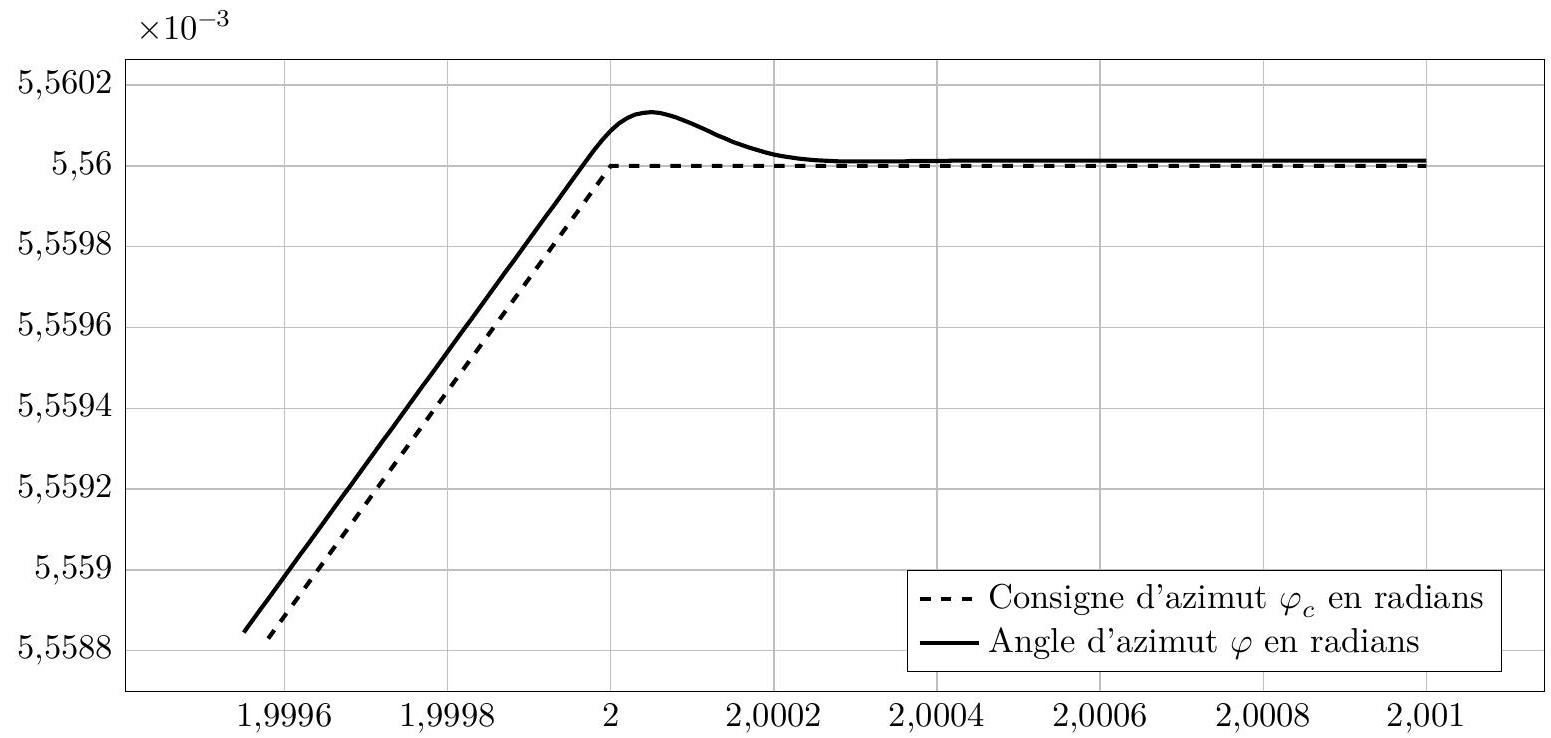
\includegraphics[width=\textwidth]{2024_12_07_51b7f57c7f055c2d8d29g-11(1)}
%
%%Figure 14 
%\caption{Simulation temporelle de l'asservissement de la figure C du document réponse avec la correction à avance de phase (zoom au voisinage de l'instant $t=T_{\mathrm{op}}=2 \mathrm{~s}$ )
%\label{CCS_MP_2017:fig_14}}
%\end{figure}
%
%%Q 25 
%\question{\label{CCS_MP_2017:q_25}En indiquant les éléments de validation par rapport aux exigences du cahier des charges, justifier qu'il est possible de réaliser des mesures en continu avec la correction à avance de phase synthétisée}
%\ifprof
%\begin{corrige}
%\end{corrige}
%\else
%\fi
%
%
%\subsection{Conclusion et perspectives de l'étude}
%\begin{obj}
%Analyser la démarche proposée dans ce sujet pour l'étude de la station totale LeICA TCRA 1103 et la comparer à la démarche de l'ingénieur abordée dans les programmes% de la filière MP
%\end{obj}
%
%La démarche de l'ingénieur abordée dans le programme de sciences industrielles de l'ingénieur de la filière MP a pour objectif de quantifier les écarts entre trois performances: voir figure \ref{CCS_MP_2017:fig_15}\\
%
%\begin{figure}[!h]
%\centering
%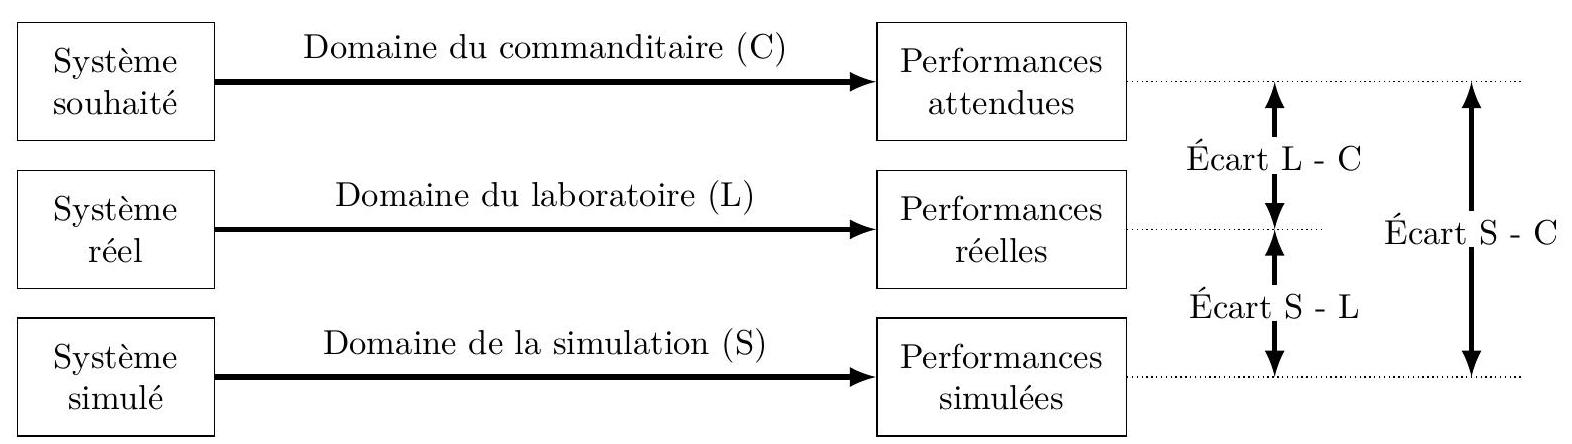
\includegraphics[width=\textwidth]{2024_12_07_51b7f57c7f055c2d8d29g-11}
%
%%Figure 15 
%\caption{Synoptique de la démarche de l'ingénieur, telle que présentée dans le programme\\
%\label{CCS_MP_2017:fig_15}}
%\end{figure}
%
%%Q 26 
%\question{\label{CCS_MP_2017:q_26}Proposer, en moins de 50 mots, une synthèse sur ce qu'il reste à faire pour finaliser la démarche de l'ingénieur telle qu'abordée en sciences industrielles de l'ingénieur}
%\ifprof
%\begin{corrige}
%\end{corrige}
%\else
%\fi


